% \documentclass[aspectratio=169, 11pt]{beamer}
\documentclass[aspectratio=169, 11pt, handout]{beamer}
 
% ── Theme ──
\usetheme{Madrid}
\usecolortheme{default}
\setbeamertemplate{navigation symbols}{}
\setbeamertemplate{footline}{%
  \leavevmode\hbox{%
    \begin{beamercolorbox}[wd=.333333\paperwidth,ht=2.5ex,dp=1ex,center]{author in head/foot}%
      \usebeamerfont{author in head/foot}\insertshortauthor
    \end{beamercolorbox}%
    \begin{beamercolorbox}[wd=.333333\paperwidth,ht=2.5ex,dp=1ex,center]{title in head/foot}%
      \usebeamerfont{title in head/foot}\insertshorttitle
    \end{beamercolorbox}%
    \begin{beamercolorbox}[wd=.333333\paperwidth,ht=2.5ex,dp=1ex,right]{date in head/foot}%
      \usebeamerfont{date in head/foot}\insertframenumber{} / \inserttotalframenumber\hspace*{2ex}
    \end{beamercolorbox}}}
 
% ── Packages ──
\usepackage{amsmath,amssymb}
\usepackage{booktabs}
\usepackage{xcolor}
\usepackage{colortbl}
\usepackage{tikz}
\usetikzlibrary{arrows.meta, positioning}
\usetikzlibrary{calc}
 
% ── Colors ──
\definecolor{sbgreen}{HTML}{00704A}
\definecolor{warnred}{HTML}{CC0000}
\definecolor{noteblue}{HTML}{2060A0}
 
% ── Commands ──
\newcommand{\E}{\mathbb{E}}
\newcommand{\Var}{\mathrm{Var}}
\newcommand{\Cov}{\mathrm{Cov}}
\newcommand{\SE}{\mathrm{SE}}
\newcommand{\Prob}{\mathrm{Pr}}
\newcommand{\indep}{\perp\!\!\!\perp}
\DeclareMathOperator{\plim}{plim}
 
% ── Reusable TikZ styles ──
\tikzset{
    tnode/.style={draw, rounded corners, fill=gray!10, minimum width=2.2cm, minimum height=0.65cm, font=\small, align=center},
    tgreen/.style={tnode, fill=sbgreen!15, draw=sbgreen},
    tblue/.style={tnode, fill=noteblue!12, draw=noteblue},
    tred/.style={tnode, fill=red!8, draw=warnred},
    tarrow/.style={-{Stealth}, thick}
}

% ── Title ──
\title[Lecture 6]{Lecture 6: Constrained Targeting}
\subtitle{Applied ML for Business Part II}
\author{Zhikun Lu}
\date{\today}

\begin{document}

% ====================================================================
\begin{frame}
\titlepage
\end{frame}

% ====================================================================
\begin{frame}{Where We Are}

\begin{center}
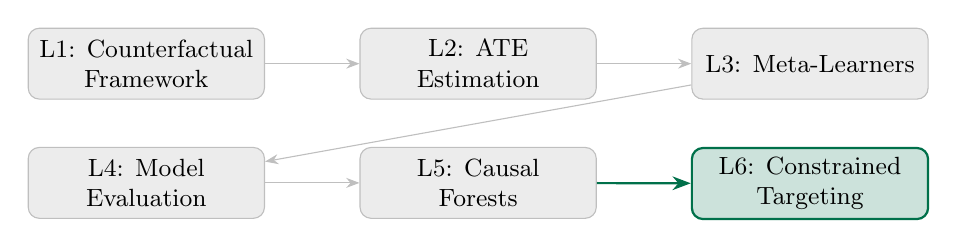
\begin{tikzpicture}[
    node distance=0.6cm and 1.2cm,
    box/.style={draw, rounded corners, minimum width=3cm, minimum height=0.9cm, font=\small, align=center},
    done/.style={box, fill=gray!15, draw=gray!50},
    active/.style={box, fill=sbgreen!20, draw=sbgreen, thick},
]
\node[done] (L1) {L1: Counterfactual\\Framework};
\node[done, right=of L1] (L2) {L2: ATE\\Estimation};
\node[done, right=of L2] (L3) {L3: Meta-Learners};
\node[done, below=of L1] (L4) {L4: Model\\Evaluation};
\node[done, below=of L2] (L5) {L5: Causal\\Forests};
\node[active, below=of L3] (L6) {L6: Constrained\\Targeting};

\draw[-{Stealth}, gray!50] (L1) -- (L2);
\draw[-{Stealth}, gray!50] (L2) -- (L3);
\draw[-{Stealth}, gray!50] (L3) -- (L4);
\draw[-{Stealth}, gray!50] (L4) -- (L5);
\draw[-{Stealth}, thick, sbgreen] (L5) -- (L6);
\end{tikzpicture}
\end{center}

\bigskip

Lectures 1--5: \emph{Estimate} $\hat{\tau}(x_i)$. \quad Lecture 6: \emph{Use} it.

\end{frame}

% ====================================================================
\begin{frame}{Today's Plan}

\textbf{From CATE to Decisions: Constrained Targeting}
\begin{enumerate}
    \item From $\hat{\tau}(x)$ to a treatment rule: maximizing business impact
    \item Budget-constrained targeting
    \item Customer-heterogeneous costs and the two-model pipeline
    \item Uncertainty 
    \item Beyond profits: fairness constraints
\end{enumerate}

\end{frame}


% %%%%%%%%%%%%%%%%%%%%%%%%%%%%%%%%%%%%%%%%%%%%%%%%%%%%%%%%%%%%%%%%%%%%
\section{From CATE to Decisions}
% %%%%%%%%%%%%%%%%%%%%%%%%%%%%%%%%%%%%%%%%%%%%%%%%%%%%%%%%%%%%%%%%%%%%

% ====================================================================
\begin{frame}{Recall: The Starbucks CATE Estimates}
 
From Lecture 5, our causal forest produces validated CATE estimates.

\medskip

\textbf{Treatment:} app push notification with a \textyen5-off coupon for a seasonal drink.

\textbf{Outcome:} purchase or not (binary, 1 or 0)

\bigskip

\begin{center}
\begin{tabular}{llccc}
\toprule
\textbf{Type} & \textbf{Spending} & $\hat{\tau}(x)$ & \textbf{Count} & \textbf{Share} \\
\midrule
Analyst   & High & 20\% & 2,500 & 25\% \\
Analyst   & Low  & 20\% & 2,500 & 25\% \\
Executive & High & 5\%  & 2,500 & 25\% \\
Executive & Low  & 5\%  & 2,500 & 25\% \\
\bottomrule
\end{tabular}
\end{center}

\bigskip

\textbf{Question:} Who should receive the notification?

\end{frame}


% ====================================================================
\begin{frame}{Step 1: Zero-Cost Treatment}

Now assume the notification does not come with a coupon.\\

\medskip

If sending the notification costs nothing, the decision rule is trivial:
\[
d^*(x_i) = \mathbf{1}\{\hat{\tau}(x_i) > 0\}
\]

\pause

\begin{center}
\begin{tabular}{llccc}
\toprule
\textbf{Type} & \textbf{Spending} & $\hat{\tau}(x)$ & $\hat{\tau} > 0$? & \textbf{Notify?} \\
\midrule
Analyst & High & 20\% & \textcolor{sbgreen}{Yes} & \textcolor{sbgreen}{Yes} \\
Analyst & Low & 20\% & \textcolor{sbgreen}{Yes} & \textcolor{sbgreen}{Yes} \\
Executive & High & 5\% & \textcolor{sbgreen}{Yes} & \textcolor{sbgreen}{Yes} \\
Executive & Low & 5\% & \textcolor{sbgreen}{Yes} & \textcolor{sbgreen}{Yes} \\
\bottomrule
\end{tabular}
\end{center}

\bigskip

All 10,000 customers get notified. Every customer is evaluated independently.

\end{frame}


% ====================================================================
\begin{frame}{Step 2: A Hidden Cost}

The data science team discovers: some notified customers \textbf{disable notifications permanently}.

\medskip

\begin{itemize}
    \item Long-term revenue loss from opt-out: \textyen150. Opt-out probability: $p_{\text{opt}} = 1\%$.
    \item Expected cost per notification: $c = 150 \times 0.01 = \text{\textyen}1.50$.
\end{itemize}

\pause
\medskip

Revenue per incremental visit: $m = \text{\textyen}30$. Threshold: $c/m = 1.50/30 = 5\%$.
\[
d^*(x_i) = \mathbf{1}\left\{\hat{\tau}(x_i) > 5\%\right\}
\]

\pause
\medskip

\begin{center}
\begin{tabular}{llccc}
\toprule
\textbf{Type} & \textbf{Spending} & $\hat{\tau}(x)$ & $\hat{\tau} > 5\%$? & \textbf{Notify?} \\
\midrule
Analyst & High/Low & 20\% & \textcolor{sbgreen}{Yes} & \textcolor{sbgreen}{Yes (5,000)} \\
Executive & High/Low & 5\% & \textcolor{warnred}{Borderline} & \textcolor{warnred}{No} \\
\bottomrule
\end{tabular}
\end{center}

\end{frame}


% ====================================================================
\begin{frame}{Step 3: Budget Constraint}

The data science team also discovers that if we send notifications at a low frequency, the opt-out rate would be significantly lower. Therefore, the product management caps notifications at \textbf{1,000 per day} to limit notification fatigue.

\bigskip

Even if all analysts pass the threshold, only 1,000 can be notified. Customers now \emph{compete}.

\pause
\bigskip

\begin{center}
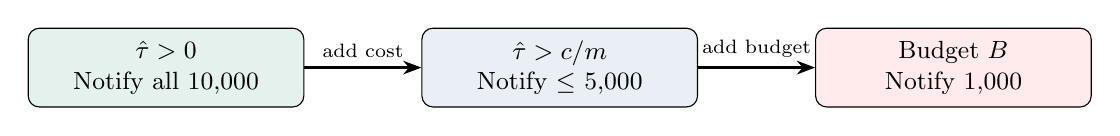
\begin{tikzpicture}[
    block/.style={draw, rounded corners, minimum width=3.5cm, minimum height=1cm, font=\small, align=center}
]
\node[block, fill=sbgreen!10] (s1) at (0,0) {$\hat{\tau} > 0$\\Notify all 10,000};
\node[block, fill=noteblue!10] (s2) at (5,0) {$\hat{\tau} > c/m$\\Notify $\leq$ 5,000};
\node[block, fill=red!8] (s3) at (10,0) {Budget $B$\\Notify 1,000};
\draw[tarrow] (s1) -- (s2) node[midway, above, font=\scriptsize]{add cost};
\draw[tarrow] (s2) -- (s3) node[midway, above, font=\scriptsize]{add budget};
\end{tikzpicture}
\end{center}

\bigskip

Each step adds one friction. The marginal customer is no longer evaluated against zero or a fixed threshold; they are evaluated against the \emph{next best alternative}.

\end{frame}


% %%%%%%%%%%%%%%%%%%%%%%%%%%%%%%%%%%%%%%%%%%%%%%%%%%%%%%%%%%%%%%%%%%%%
\section{Budget-Constrained Targeting}
% %%%%%%%%%%%%%%%%%%%%%%%%%%%%%%%%%%%%%%%%%%%%%%%%%%%%%%%%%%%%%%%%%%%%

% ====================================================================
\begin{frame}{The Budget-Constrained Problem}

At this stage, cost $c = \text{\textyen}1.50$ is \textbf{uniform} across customers (same opt-out risk for everyone).

\begin{block}{Optimization}
\vspace{-0.5em}
\[
\max_{d_1, \ldots, d_n \in \{0,1\}} \sum_{i=1}^{n} d_i \cdot \bigl[\hat{\tau}(x_i) \cdot m - c\bigr] \qquad \text{subject to} \quad \sum_{i=1}^{n} d_i \leq B
\]
\end{block}

\pause
\bigskip

The objective is \textbf{separable} in $d_i$. The solution is sorting:

\begin{enumerate}
    \item Compute net value: $v_i = \hat{\tau}(x_i) \cdot m - c$ for each customer.
    \item Rank by $v_i$ in decreasing order.
    \item Treat the top $\min(B,\; |\{i : v_i > 0\}|)$ customers.
\end{enumerate}

\pause
\bigskip

When cost is uniform, ranking by $v_i$ is the same as ranking by $\hat{\tau}(x_i)$.

\end{frame}


% ====================================================================
\begin{frame}{Starbucks: Budget = 1,000 Notifications}

The causal forest reveals finer heterogeneity within the analyst group:

\bigskip

\begin{center}
\begin{tabular}{lcccc}
\toprule
\textbf{Rank} & \textbf{Segment} & $\hat{\tau}(x)$ & $v_i = \hat{\tau} \cdot 30 - 1.50$ & \textbf{Notify?} \\
\midrule
1--800 & High-response analysts & 25\% & \textyen6.00 & \textcolor{sbgreen}{Yes} \\
801--1,200 & Moderate analysts & 18\% & \textyen3.90 & \textcolor{sbgreen}{Top 200 only} \\
1,201--5,000 & Other analysts & 12\% & \textyen2.10 & \textcolor{warnred}{No (budget)} \\
5,001--10,000 & Executives & 5\% & \textyen0.00 & \textcolor{warnred}{No} \\
\bottomrule
\end{tabular}
\end{center}

\pause
\bigskip

Budget binds at 1,000: all 800 high-response + 200 of the 400 moderate analysts.

\medskip

Note: even the remaining analysts and executives have $v_i \geq 0$, but the budget excludes them. The constraint, not the threshold, is the binding friction.

\end{frame}


% %%%%%%%%%%%%%%%%%%%%%%%%%%%%%%%%%%%%%%%%%%%%%%%%%%%%%%%%%%%%%%%%%%%%
\section{Customer-Heterogeneous Costs}
% %%%%%%%%%%%%%%%%%%%%%%%%%%%%%%%%%%%%%%%%%%%%%%%%%%%%%%%%%%%%%%%%%%%%
 
% ====================================================================
\begin{frame}{Why Costs Are Not Uniform}
 
So far: every notification costs the same (\textyen1.50 opt-out risk). But the \textyen5 coupon creates an additional cost that varies by customer.
 
\pause
\smallskip
 
\textbf{Key insight:} the coupon is redeemed only upon purchase, so:
\vspace{-0.5em}
\[
\hat{c}(x_i) = \underbrace{1.50}_{\text{opt-out}} + \underbrace{5 \times \Prob(Y(1)\!=\!1 \mid X_i)}_{\text{expected coupon payout}} \qquad v_i = \hat{\tau}(x_i) \cdot m - \hat{c}(x_i)
\]
\vspace{-0.8em}
 
\pause
 
\begin{center}
\small
\begin{tabular}{llcccccl}
\toprule
\textbf{Type} & \textbf{Spend} & $\hat{\tau}$ & $\Prob(Y_0\!=\!1)$ & $\Prob(Y_1\!=\!1)$ & $\hat{c}(x)$ & $v_i$ & \textbf{Treat?} \\
\midrule
Analyst & Low  & 20\% & 0\% & 20\% & \textyen2.50 & \textyen3.50 & \textcolor{sbgreen}{Yes} \\
Analyst & High & 20\% & 30\% & 50\% & \textyen4.00 & \textyen2.00 & \textcolor{sbgreen}{Yes} \\
Exec & Low  & 5\% & 30\% & 35\% & \textyen3.25 & $-$\textyen1.75 & \textcolor{warnred}{No} \\
Exec & High & 5\% & 60\% & 65\% & \textyen4.75 & $-$\textyen3.25 & \textcolor{warnred}{No} \\
\bottomrule
\end{tabular}
\end{center}
 
\pause
\smallskip
 
Under \textbf{uniform cost}, spending was irrelevant. Under \textbf{heterogeneous cost}, all four segments separate: high baseline $\Prob(Y_0\!=\!1)$ drives up cost.
 
\end{frame}
 
 
% ====================================================================
\begin{frame}{Why Are High Spenders Expensive?}
 
The same net value admits a revealing decomposition:
\vspace{-0.8em}
\[
v_i = \underbrace{\hat{\tau}(x_i) \cdot (m - 5)}_{\substack{\text{incremental buyers:}\\\text{margin minus coupon}}} \;-\; \underbrace{5 \cdot \Prob(Y(0)\!=\!1 \mid X_i)}_{\substack{\text{baseline buyers:}\\\text{coupon, no new revenue}}} \;-\; 1.50
\]
\vspace{-1.0em}
 
\pause
 
The second term is the \textbf{sure-thing cost}: customers who would have purchased anyway redeem the coupon for free.
 
\smallskip
 
\begin{center}
\small
\begin{tabular}{llcccc}
\toprule
\textbf{Type} & \textbf{Spend} & $\hat{\tau}\!\cdot\!25$ & $5 \!\times\! \Prob(Y_0\!=\!1)$ & $- 1.50$ & $v_i$ \\
\midrule
Analyst & Low  & \textyen5.00 & \textyen0.00 & $-$\textyen1.50 & \textyen3.50 \\
Analyst & High & \textyen5.00 & \textyen1.50 & $-$\textyen1.50 & \textyen2.00 \\
Executive & Low  & \textyen1.25 & \textyen1.50 & $-$\textyen1.50 & $-$\textyen1.75 \\
Executive & High & \textyen1.25 & \textyen3.00 & $-$\textyen1.50 & $-$\textyen3.25 \\
\bottomrule
\end{tabular}
\end{center}
\vspace{-0.5em}
 
\pause
 
Analyst-Low has zero sure-thing cost (nobody buys without the coupon). Analyst-High loses \textyen1.50 to baseline buyers. Same CATE, different profitability.
 
\pause
\vspace{0.2em}
 
\textbf{Note:} $\hat{c}(x_i) = 1.50 + 5 \!\times\! \Prob(Y(1)\!=\!1)$ gives the same $v_i$. The two formulas are algebraically equivalent; use whichever builds the right intuition.
 
\end{frame}
 
 
 
% ====================================================================
\begin{frame}{The Two-Model Pipeline}
 
With customer-heterogeneous costs, targeting requires \textbf{two} ML models:
 
\bigskip
 
\begin{enumerate}
    \item \textbf{Benefit model} (causal): estimate $\hat{\tau}(x_i)$ from the experiment.
    
    Requires counterfactual reasoning (Lectures 1--5).
    
    \medskip
    
    \item \textbf{Cost model} (predictive): estimate $\hat{c}(x_i)$ from past campaign data.
    
    Standard supervised learning: predict $\Prob(Y(1)\!=\!1 \mid X)$ from treated observations. Or equivalently, predict $\Prob(Y(0)\!=\!1 \mid X)$ from control observations, then add $\hat{\tau}(x_i)$.
\end{enumerate}
 
\pause
\bigskip
 
The causal/predictive distinction matters:
\begin{itemize}
    \item Benefit side requires experimental or quasi-experimental data.
    \item Cost side can use observational data from past campaigns.
\end{itemize}
 
\pause
\bigskip
 
Different estimation tasks, different data requirements.
 
\end{frame}
 
 
% ====================================================================
\begin{frame}{Without a Budget: Customer-Specific Thresholds}
 
With no budget constraint, each customer is evaluated independently, but the threshold is now \emph{customer-specific}:
\[
d^*(x_i) = \mathbf{1}\bigl\{\hat{\tau}(x_i) \cdot m > \hat{c}(x_i)\bigr\}
\]
 
\pause
\bigskip
 
\begin{center}
\begin{tabular}{llccccl}
\toprule
\textbf{Type} & \textbf{Spend} & $\hat{\tau}$ & $\hat{\tau}\!\cdot\!30$ & $\hat{c}(x)$ & Net & \textbf{Treat?} \\
\midrule
Analyst & Low  & 20\% & \textyen6.00 & \textyen2.50 & \textyen3.50 & \textcolor{sbgreen}{Yes} \\
Analyst & High & 20\% & \textyen6.00 & \textyen4.00 & \textyen2.00 & \textcolor{sbgreen}{Yes} \\
Executive & Low  & 5\% & \textyen1.50 & \textyen3.25 & $-$\textyen1.75 & \textcolor{warnred}{No} \\
Executive & High & 5\% & \textyen1.50 & \textyen4.75 & $-$\textyen3.25 & \textcolor{warnred}{No} \\
\bottomrule
\end{tabular}
\end{center}
 
\pause
\bigskip
 
Both analyst segments pass; both executive segments fail. But the \textbf{net values differ}: Analyst-Low generates \textyen3.50 per customer vs.\ Analyst-High at \textyen2.00. The prognostic variable now matters for ranking.
 
\end{frame}
 
 
% ====================================================================
\begin{frame}{How Much Will the Campaign Cost?}
 
The firm treats all 5,000 analysts. Expected total cost:
\[
\hat{\mu}_C = 2{,}500 \times 4.00 + 2{,}500 \times 2.50 = \text{\textyen}16{,}250
\]
 
\pause
\medskip
 
But realized cost is random. Each customer either redeems (\textyen6.50) or not (\textyen1.50). If redemption runs higher than predicted, actual cost exceeds the estimate.
 
\pause
\medskip
 
Finance asks: ``What is the chance we exceed \textyen18,000?''
 
\medskip
 
Under a normal approximation for total cost:
\[
\Prob\!\left(\sum_{i} d_i \cdot c_i > C\right) \leq \alpha \quad \Longleftrightarrow \quad \hat{\mu}_C + z_\alpha \hat{\sigma}_C \leq C
\]
 
\pause
\medskip
 
Even without a hard budget cap, the firm wants to control spending risk. The safety margin $z_\alpha \hat{\sigma}_C$ gives finance a confidence interval on total campaign cost.
 
\end{frame}
 
 
% ====================================================================
\begin{frame}{With a Budget: The Knapsack Problem}
 
Now finance imposes a hard cap: total campaign cost $\leq C$.
 
\bigskip
 
With heterogeneous costs, this is a \textbf{knapsack}:
\[
\max_{d_1, \ldots, d_n} \sum_{i=1}^{n} d_i \cdot \hat{\tau}(x_i) \cdot m \qquad \text{subject to} \quad \sum_{i=1}^{n} d_i \cdot \hat{c}(x_i) \leq C
\]
 
\pause
\bigskip
 
The greedy solution: rank by the \textbf{benefit-cost ratio}:
\[
r_i = \frac{\hat{\tau}(x_i) \cdot m}{\hat{c}(x_i)}
\]
and treat in decreasing order of $r_i$ until the budget is exhausted.
 
\pause
\bigskip
 
With uniform costs, ranking by $r_i$ reduces to ranking by $\hat{\tau}(x_i)$, so spending was irrelevant. With heterogeneous costs, spending enters through $\hat{c}(x_i)$ and changes the ranking.
 
\end{frame}
 
 
% ====================================================================
\begin{frame}{Knapsack: Starbucks Numerics}
 
\begin{center}
\begin{tabular}{llccccc}
\toprule
\textbf{Type} & \textbf{Spend} & $\hat{\tau}$ & $\hat{\tau}\!\cdot\!30$ & $\hat{c}(x)$ & $r_i$ & \textbf{Rank} \\
\midrule
Analyst & Low  & 20\% & \textyen6.00 & \textyen2.50 & 2.40 & \textcolor{sbgreen}{1st} \\
Analyst & High & 20\% & \textyen6.00 & \textyen4.00 & 1.50 & 2nd \\
Executive & Low  & 5\% & \textyen1.50 & \textyen3.25 & 0.46 & 3rd \\
Executive & High & 5\% & \textyen1.50 & \textyen4.75 & 0.32 & 4th \\
\bottomrule
\end{tabular}
\end{center}
 
\pause
\bigskip
 
\textbf{Under uniform cost:} all analysts tied, all executives tied.
 
\textbf{Under heterogeneous cost:} Analyst-Low dominates Analyst-High. Same CATE, half the cost.
 
\pause
\bigskip
 
Under a tight budget, the firm should exhaust all low-spending analysts before moving to high-spending analysts. The prognostic variable that was irrelevant for estimation becomes decisive for allocation.
 
\end{frame}
 
 
% ====================================================================
\begin{frame}{Budget Safety Under Heterogeneous Costs}
 
The knapsack uses expected costs $\hat{c}(x_i)$. Realized costs are random.
 
\medskip
 
To control budget overrun at tolerance $\alpha$, shrink the effective budget:
\[
\sum_{i} d_i \cdot \hat{c}(x_i) \;\leq\; C - z_\alpha \cdot \hat{\sigma}_C
\]
 
\pause
\medskip
 
Suppose we target all 2,500 Analyst-Low ($\hat{p}_{\text{red}} = 0.20$) and 2,500 Analyst-High ($\hat{p}_{\text{red}} = 0.50$):
\begin{align*}
\hat{\sigma}_C &= \sqrt{2{,}500 \times 25 \times 0.20 \times 0.80 \;+\; 2{,}500 \times 25 \times 0.50 \times 0.50} \\
&= \sqrt{10{,}000 + 15{,}625} = \sqrt{25{,}625} \approx \text{\textyen}160
\end{align*}
 
\pause
 
Safety margin (5\%): $1.645 \times 160 \approx \text{\textyen}263$. The firm reserves \textyen263 as a buffer.
 
\medskip
 
Note: a better cost model (lower $\hat{\sigma}^2$) $\Rightarrow$ smaller margin $\Rightarrow$ more customers treated.
 
\end{frame}
 
 
% %%%%%%%%%%%%%%%%%%%%%%%%%%%%%%%%%%%%%%%%%%%%%%%%%%%%%%%%%%%%%%%%%%%%
\section{Benefit-Side Uncertainty}
% %%%%%%%%%%%%%%%%%%%%%%%%%%%%%%%%%%%%%%%%%%%%%%%%%%%%%%%%%%%%%%%%%%%%
 
% ====================================================================
\begin{frame}{The Other Side: Noisy CATE Estimates}
 
So far we treated $\hat{\tau}(x_i)$ as known. But CATE estimates are noisy.
 
\medskip
 
\textbf{Conservative rule:} replace the point estimate with a lower confidence bound:
\[
d^*(x_i) = \mathbf{1}\left\{\hat{\tau}(x_i) - z_\alpha \cdot \widehat{\SE}(x_i) > \frac{c(x_i)}{m}\right\}
\]
 
\pause
\medskip
 
\begin{center}
\small
\begin{tabular}{llccccc}
\toprule
\textbf{Type} & \textbf{Spend} & $\hat{\tau}$ & $\widehat{\SE}$ & LB & $c_i/m$ & \textbf{Treat?} \\
\midrule
Analyst & Low  & 20\% & 5\% & 11.8\% & 8.3\% & \textcolor{sbgreen}{Yes} \\
Analyst & High & 20\% & 3\% & 15.1\% & 13.3\% & \textcolor{sbgreen}{Yes} \\
Exec & Low  & 5\% & 4\% & $-$1.6\% & 10.8\% & \textcolor{warnred}{No} \\
Exec & High & 5\% & 3\% & 0.1\% & 15.8\% & \textcolor{warnred}{No} \\
\bottomrule
\end{tabular}
\end{center}
 
\pause
\medskip
 
This is \emph{why} we needed valid CIs from causal forests (Lecture 5): they feed directly into the targeting decision.
 
\end{frame}
 
 
% ====================================================================
\begin{frame}{The Dissatisfaction with $z_\alpha$}
 
The conservative rule has a tuning parameter $z_\alpha$ reflecting \emph{subjective risk preference}:
 
\begin{itemize}
    \item $z_\alpha = 0$: use the point estimate (risk-neutral).
    \item $z_\alpha = 1.96$: require 95\% confidence (very conservative).
\end{itemize}
 
\pause
\bigskip
 
How should the marketing team choose $z_\alpha$? There is no principled answer from the data alone.
 
\pause
\bigskip
 
\textbf{Contrast with the newsvendor} (Module 1): the cost ratio $c_u/(c_u + c_o)$ pinned down the optimal quantile through business primitives alone. Nothing was left for the modeler to choose.
 
\medskip
 
Can we get the same structure on the causal side?
 
\end{frame}
 
 
% ====================================================================
\begin{frame}{From Customers to Stores}
 
So far we targeted individual customers. Now consider a different level of decision.
 
\bigskip
 
Starbucks HQ decides which \emph{stores} should run a BOGO promotion.
 
\bigskip
 
Each store has:
\begin{itemize}
    \item Baseline demand: $d_0 = 200$ drinks/day.
    \item Barista capacity: $q = 210$ drinks/day.
    \item Capacity slack: $s = q - d_0 = 10$ drinks.
\end{itemize}
 
\pause
\bigskip
 
If the promotion lifts demand by $\delta$ drinks:
\begin{itemize}
    \item $\delta \leq 10$: every extra drink sells at margin $p = \text{\textyen}25$. \hfill (upside)
    \item $\delta > 10$: excess customers face long waits, leave frustrated. Goodwill cost $g = \text{\textyen}15$ per lost customer. \hfill (downside)
\end{itemize}
 
\end{frame}
 
 
% ====================================================================
\begin{frame}{The Newsvendor Structure in Promotion Targeting}
 
Incremental profit from promoting a store:
\[
V(\delta) = \underbrace{p \cdot \min(\delta,\, s)}_{\text{revenue from extra drinks}} \;-\; \underbrace{g \cdot (\delta - s)^+}_{\text{goodwill loss from overflow}} \;-\; c
\]
 
\pause
\bigskip
 
A \textbf{two-piece linear function} in $\delta$ with a kink at the capacity slack $s$:
 
\medskip
 
\begin{center}
\begin{tabular}{lcl}
Below slack ($\delta < s$): & marginal value $= +p = +\text{\textyen}25$ & (sell another drink) \\
Above slack ($\delta > s$): & marginal value $= -g = -\text{\textyen}15$ & (lose a customer) \\
\end{tabular}
\end{center}
 
\pause
\bigskip
 
The same structure as the newsvendor:
\begin{itemize}
    \item Capacity slack $s$ $\longleftrightarrow$ stocking quantity $q$
    \item Treatment effect $\delta$ $\longleftrightarrow$ realized demand $D$
    \item Drink margin $p$ $\longleftrightarrow$ underage cost $c_u$
    \item Goodwill cost $g$ $\longleftrightarrow$ overage cost $c_o$
\end{itemize}
 
\end{frame}
 
 
% ====================================================================
\begin{frame}{Why the CATE Is Not Enough}
 
Two stores in analyst-heavy neighborhoods. Both have $\E[\delta \mid x] = 15$ extra drinks. Slack $s = 10$.
 
\bigskip
 
\textbf{Store A} (steady neighborhood): $\delta = 15$ with certainty.
\begin{align*}
V &= 25 \times \min(15, 10) - 15 \times (15 - 10)^+ - c = 250 - 75 - c = 175 - c
\end{align*}
 
Promote if $c < 175$. \textcolor{sbgreen}{Almost certainly yes.}
 
\pause
\bigskip
 
\textbf{Store B} (volatile neighborhood): $\delta = 30$ w.p.\ 0.5, $\;\delta = 0$ w.p.\ 0.5.
\begin{align*}
\E[V] &= 25 \times \underbrace{\E[\min(\delta, 10)]}_{=5} - 15 \times \underbrace{\E[(\delta - 10)^+]}_{=10} - c = 125 - 150 - c = -25 - c
\end{align*}
 
\textcolor{warnred}{Never promote}, regardless of $c$.
 
\pause
\bigskip
 
Same CATE. Opposite decisions. The \emph{shape} of the treatment effect distribution around the capacity constraint is decisive.
 
\end{frame}
 
 
% ====================================================================
\begin{frame}{The Critical Fractile}
 
The expected profit can be rewritten using the \textbf{pinball loss} $\rho_\tau$:
\[
\E[V(\delta) \mid x] + c = -(p + g) \cdot \E\bigl[\rho_\tau(\delta - s) \mid x\bigr]
\]
 
where the critical fractile is:
\[
\tau^* = \frac{p}{p + g} = \frac{25}{25 + 15} = 0.625
\]
 
\pause
\bigskip
 
The decision depends on the \textbf{62.5th percentile} of the treatment effect distribution, not the mean. Pinned entirely by business primitives ($p$ and $g$). No subjective $z_\alpha$.
 
\pause
\bigskip
 
\textbf{The parallel to Module 1 is exact:}
\begin{itemize}
    \item Newsvendor: $c_u/(c_u + c_o)$ $\to$ quantile of the \emph{demand} distribution.
    \item Promotion targeting: $p/(p + g)$ $\to$ quantile of the \emph{treatment effect} distribution.
\end{itemize}
 
\medskip
 
Estimating this requires a \textbf{Conditional Quantile Treatment Effect} (CQTE), not a CATE.
 
\end{frame}
 
 
% %%%%%%%%%%%%%%%%%%%%%%%%%%%%%%%%%%%%%%%%%%%%%%%%%%%%%%%%%%%%%%%%%%%%
\section{Fairness Constraints}
% %%%%%%%%%%%%%%%%%%%%%%%%%%%%%%%%%%%%%%%%%%%%%%%%%%%%%%%%%%%%%%%%%%%%
 
% ====================================================================
\begin{frame}{From Efficiency to Equity}
 
Return to individual-level targeting with the budget-constrained policy ($B = 1{,}000$).
 
\bigskip
 
The optimizer does not use gender. But the resulting policy correlates with it:
 
\begin{center}
\begin{tabular}{lcccc}
\toprule
& \textbf{Female} & \textbf{Male} & \textbf{Total} \\
\midrule
Analysts (high CATE) & 1,500 & 3,500 & 5,000 \\
Executives (low CATE) & 3,500 & 1,500 & 5,000 \\
\midrule
Total & 5,000 & 5,000 & 10,000 \\
\bottomrule
\end{tabular}
\end{center}
 
\pause
\bigskip
 
The optimal policy treats mostly analysts. Since analysts are disproportionately male (70\%), the policy treats more men than women.
 
\medskip
 
Suppose the top 1,000 by $v_i$ contains 750 men and 250 women.
 
Treatment rates: $750/5{,}000 = 15\%$ (male) vs.\ $250/5{,}000 = 5\%$ (female). A \textbf{3:1 disparity}.
 
\end{frame}
 
 
% ====================================================================
\begin{frame}{Group Treatment Parity}
 
Require treatment rates to stay within a factor $\gamma \geq 1$:
\[
\max_{d_1, \ldots, d_n} \sum_{i} d_i \cdot v_i \quad \text{s.t.} \quad \sum_i d_i \leq B, \qquad \frac{\bar{d}_k}{\bar{d}_\ell} \leq \gamma \quad \forall\, k, \ell
\]
 
\pause
\bigskip
 
A concrete anchor: the \textbf{four-fifths rule} from U.S.\ employment law.
 
\medskip
 
The selection rate of any group must be at least 80\% of the most-selected group:
$\gamma = 1/0.8 = 1.25$.
 
\pause
\bigskip
 
The solution decomposes:
\begin{enumerate}
    \item Within each gender group, rank by $v_i$ (the ordering is preserved).
    \item Search over feasible group-level counts $(n_F, n_M)$ satisfying budget + ratio constraints.
    \item Choose the allocation that maximizes total value.
\end{enumerate}
 
\end{frame}
 
 
% ====================================================================
\begin{frame}{Fair Targeting: Starbucks Numerics}
 
Budget $B = 1{,}000$. Fairness: $\gamma \leq 1.25$. Groups: $|G_F| = 5{,}000$, $|G_M| = 5{,}000$.
 
\bigskip
 
Setting $\bar{d}_F = p$, so $\bar{d}_M \leq 1.25\,p$. The budget constraint:
 
\[
5{,}000 \times p + 5{,}000 \times 1.25\,p = 11{,}250\,p \leq 1{,}000 \implies p \approx 8.9\%
\]
 
\pause
\bigskip
 
\begin{center}
\begin{tabular}{lccc}
\toprule
\textbf{Group} & \textbf{Unconstrained} & \textbf{Fair ($\gamma = 1.25$)} & \textbf{Rate} \\
\midrule
Female & 250 & 444 & 8.9\% \\
Male & 750 & 556 & 11.1\% \\
\midrule
Total & 1,000 & 1,000 & \\
\bottomrule
\end{tabular}
\end{center}
 
\pause
\bigskip
 
The fair policy shifts $\sim$200 notifications from men to women. Total expected profit falls, but the treatment rate ratio drops from 3:1 to 1.25:1.
 
\end{frame}
 
 
% ====================================================================
\begin{frame}{The Price of Fairness}
 
The fairness constraint restricts the feasible set:
\[
\text{PoF}(\gamma) = \Pi^*_{\text{unconstrained}} - \Pi^*_{\text{fair}}(\gamma)
\]
 
\pause
\bigskip
 
The \textbf{Lagrange multiplier} on the binding fairness constraint:
 
\medskip
 
Marginal profit lost per unit tightening of $\gamma$.
 
\pause
\bigskip
 
If the multiplier is \textyen500, then reducing $\gamma$ from 1.25 to 1.20 costs roughly:
\[
0.05 \times 500 = \text{\textyen}25 \text{ in expected profit}
\]
 
\medskip
 
This gives managers a \emph{concrete number} for the equity-efficiency tradeoff.
 
\pause
\bigskip
 
Alternative fairness criteria exist (benefit parity, outcome parity), each with a different constraint and a different price. The choice is normative, not statistical.
 
\end{frame}
 
 
% %%%%%%%%%%%%%%%%%%%%%%%%%%%%%%%%%%%%%%%%%%%%%%%%%%%%%%%%%%%%%%%%%%%%
\section{The Big Picture}
% %%%%%%%%%%%%%%%%%%%%%%%%%%%%%%%%%%%%%%%%%%%%%%%%%%%%%%%%%%%%%%%%%%%%
 
% ====================================================================
\begin{frame}{Estimate-then-Optimize}
 
The targeting pipeline is a causal instance of \textbf{Predict-then-Optimize}:
 
\bigskip
 
\begin{center}
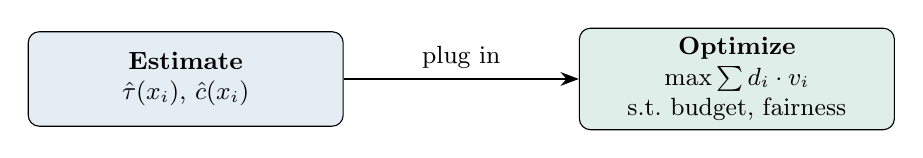
\begin{tikzpicture}[
    block/.style={draw, rounded corners, minimum width=4cm, minimum height=1.2cm, font=\small, align=center},
]
\node[block, fill=noteblue!12] (est) at (0,0) {\textbf{Estimate}\\$\hat{\tau}(x_i)$, $\hat{c}(x_i)$};
\node[block, fill=sbgreen!12] (opt) at (7,0) {\textbf{Optimize}\\$\max \sum d_i \cdot v_i$\\s.t.\ budget, fairness};
\draw[tarrow] (est) -- (opt) node[midway, above, font=\small]{plug in};
\end{tikzpicture}
\end{center}
 
\pause
\bigskip
 
\begin{center}
\small
\begin{tabular}{lcc}
\toprule
& \textbf{Module 1} & \textbf{Module 2} \\
\midrule
Predict / Estimate & Demand $\hat{D}(x)$ & CATE $\hat{\tau}(x)$ \\
Optimize & Newsvendor: choose $q^*$ & Targeting: choose $d^*$ \\
Key quantity & $F^{-1}_D(\tau)$ & Quantile of $\delta \mid x$ \\
\bottomrule
\end{tabular}
\end{center}
 
\medskip
 
The quantile CATE section shows these are the \emph{same mathematical structure}.
 
\end{frame}
 
 
% ====================================================================
\begin{frame}{SUTVA and Its Limits}
 
Everything today assumes \textbf{SUTVA}: each customer's treatment effect is independent of who else is treated.
 
\bigskip
 
This can fail at Starbucks:
\begin{itemize}
    \item \textbf{Positive spillover:} a notified customer tells a friend about the seasonal drink.
    \item \textbf{Negative spillover:} a promotion at one store shifts demand from nearby stores.
    \item \textbf{Capacity interaction:} targeting too many customers near the same store causes congestion (the newsvendor section!).
\end{itemize}
 
\pause
\bigskip
 
When interference is present, the optimal policy depends on the \emph{entire assignment vector}, not just individual CATEs. Individual-level CATE targeting is an approximation when spillovers exist.
 
\end{frame}
 
 
% ====================================================================
\begin{frame}{Extension: Multiple Treatments}
 
Today we fixed the treatment (one \textyen5-off coupon). A natural extension: \textbf{choose which offer to give each customer}.
 
\bigskip
 
\begin{itemize}
    \item Plain notification, \textyen5-off coupon, \textyen15-off coupon, BOGO, free size upgrade, \ldots
    \item Each type $t$ has its own cost $c_t$ and CATE function $\tau_t(x)$.
    \item Decision: $t^*(x_i) = \arg\max_t [\tau_t(x_i) \cdot m - c_t]$, or do not treat.
\end{itemize}
 
\pause
\bigskip
 
\textbf{Estimation extends naturally:}
\begin{itemize}
    \item S-Learner / T-Learner: encode multiple arms straightforwardly.
    \item GRF: \texttt{multi\_arm\_causal\_forest} estimates $K-1$ contrasts jointly, splitting on heterogeneity across the \emph{vector} of treatment effects.
\end{itemize}
 
\pause
\bigskip
 
The progressive ladder from today (budget $\to$ heterogeneous costs $\to$ uncertainty $\to$ fairness) carries over, with richer structure at each step.
 
\end{frame}
 
 
% %%%%%%%%%%%%%%%%%%%%%%%%%%%%%%%%%%%%%%%%%%%%%%%%%%%%%%%%%%%%%%%%%%%%
\section{Summary}
% %%%%%%%%%%%%%%%%%%%%%%%%%%%%%%%%%%%%%%%%%%%%%%%%%%%%%%%%%%%%%%%%%%%%
 
% ====================================================================
\begin{frame}{The Progressive Ladder}
 
\begin{center}
\small
\begin{tabular}{p{4.5cm}p{4cm}p{4cm}}
\toprule
\textbf{Problem} & \textbf{Decision rule} & \textbf{What it adds} \\
\midrule
Free notification & $\hat{\tau}(x) > 0$ & Baseline \\[0.3em]
Opt-out cost (uniform) & $\hat{\tau}(x) > c/m$ & Threshold \\[0.3em]
Notification cap & Rank by $\hat{\tau}$, top $B$ & Competition \\[0.3em]
Customer-specific costs & $\hat{\tau} \cdot m > \hat{c}(x_i)$ & Two-model pipeline \\[0.3em]
Budget + heterog.\ costs & Rank by $r_i$, knapsack & Benefit-cost ratio \\[0.3em]
Cost uncertainty & Safety margin $z_\alpha \hat{\sigma}_C$ & Budget buffer \\[0.3em]
Benefit uncertainty & Lower CI bound & Conservative targeting \\[0.3em]
Capacity constraint & Quantile of $\delta$ & Newsvendor / CQTE \\[0.3em]
Fairness & Group-specific thresholds & Price of fairness \\
\bottomrule
\end{tabular}
\end{center}
 
\end{frame}
 
 
% ====================================================================
\begin{frame}{Key Takeaways}
 
\begin{enumerate}
    \item \textbf{CATE estimation is not the end goal.} The decision rule is. The structure of the decision problem determines what to estimate.
 
    \pause
    \smallskip
 
    \item \textbf{Prognostic variables resurface on the cost side.} Spending and type were separable for $\hat{\tau}$ (only type mattered). On the cost side, both drive $\Prob(Y(0)\!=\!1)$ and hence $\hat{c}(x_i)$, giving all four segments different targeting priorities.
 
    \pause
    \smallskip
 
    \item \textbf{Uncertainty on both sides.} Cost-side: safety margin protects the budget. Benefit-side: conservative targeting uses CIs from causal forests. With capacity constraints, the critical fractile pins down the right quantile from business primitives alone.
 
    \pause
    \smallskip
 
    \item \textbf{Fairness has a measurable price.} The CATE-optimal policy may have disparate impact on protected groups. The Lagrange multiplier quantifies the equity-efficiency tradeoff.
\end{enumerate}
 
\end{frame}
 
 
% ====================================================================
\begin{frame}{Discussion}
 
Your Starbucks team has:
\begin{itemize}
    \item A validated causal forest for the \textyen5-off coupon notification.
    \item A redemption cost model trained on past campaign data.
    \item A daily notification cap of 1,000 and a monetary budget of \textyen8,000.
    \item A four-fifths rule on gender treatment rates.
\end{itemize}
 
\bigskip
 
\begin{enumerate}
    \item Walk through the full pipeline: what do you estimate, how do you rank customers, and which constraints bind first?
 
    \pause
    \bigskip
 
    \item The causal forest has wider CIs for women (fewer female analysts in the experimental sample). How does this interact with the conservative targeting rule and the fairness constraint?
 
    \pause
    \bigskip
 
    \item The CFO asks: ``What is the cost of the fairness policy?'' How do you produce this number?
\end{enumerate}
 
\end{frame}
 
\end{document}